\documentclass[a4paper]{article}
\usepackage[utf8]{inputenc}
\usepackage[russian,english]{babel}
\usepackage[T2A]{fontenc}
\usepackage[left=10mm, top=20mm, right=18mm, bottom=15mm, footskip=10mm]{geometry}
\usepackage{indentfirst}
\usepackage{amsmath,amssymb}
\usepackage[italicdiff]{physics}
\usepackage{graphicx}
\usepackage{multirow}
\usepackage{svg}
\graphicspath{{images/}}
\DeclareGraphicsExtensions{.pdf,.png,.jpg}
\usepackage{wrapfig}
\usepackage{caption}
\captionsetup[figure]{name=Рисунок}
\captionsetup[table]{name=Таблица}
\title{\underline{Изучение плазмы газового разряда в неоне}}
\author{Каспаров Николай, Б01-304}

\begin{document}

\maketitle
\begin{center}
\Large{\textbf{ }}
\end{center}

\subparagraph{Цель работы:}

\begin{itemize}
\item изучить спектральный состав периодических электрических сигналов
\end{itemize}

\section{Ход работы}

\subsection{Настройка генерации прямоугольных импульсов и анализ их спектра}

Частота повторения импульсов: $\nu = 1$ кГц

Длительность импульса: $\tau = T / 20 = 50$ мкс

\begin{figure}[h!]
    \centering
    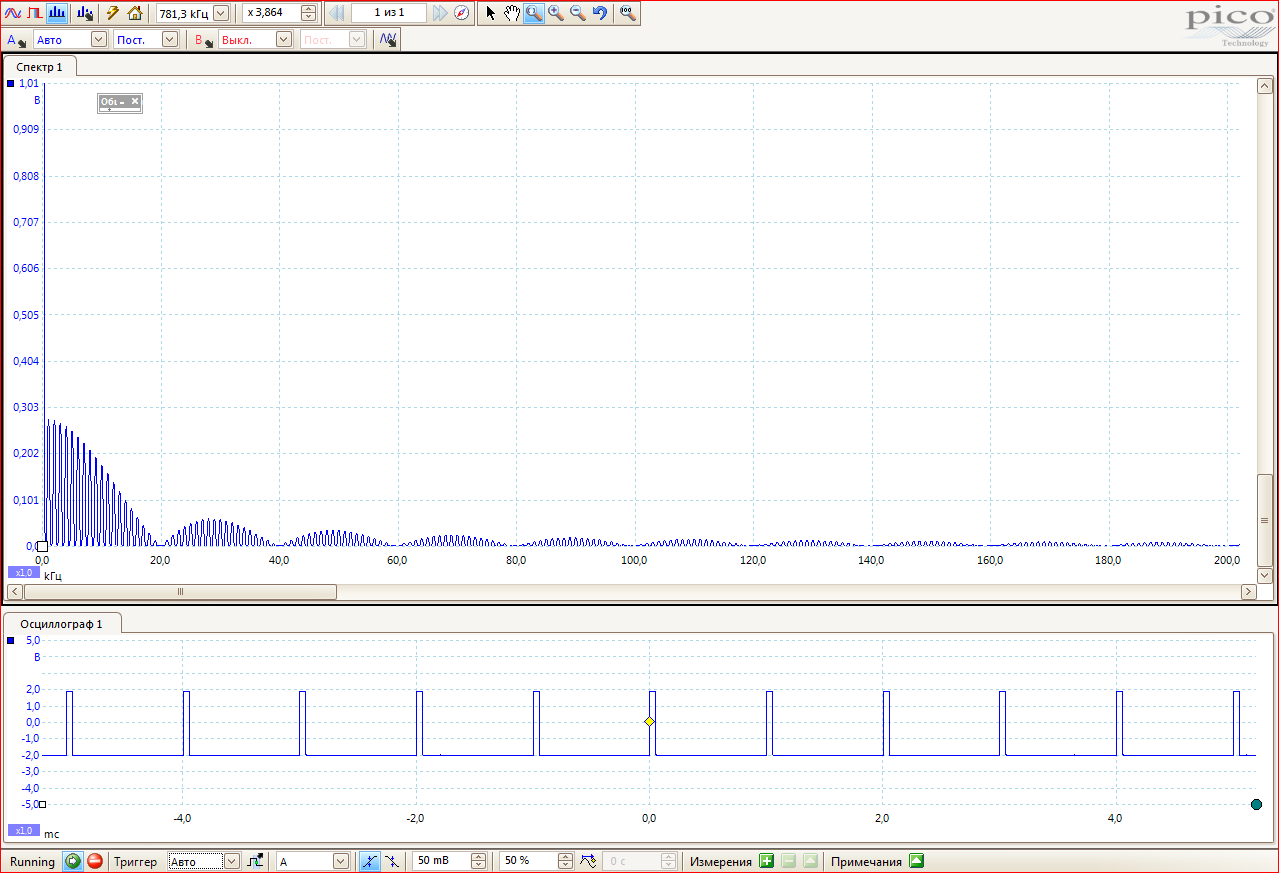
\includegraphics[width=0.5\pdfpagewidth]{Rect1.png}
    \caption{Прямоугольный сигнал 2 кГц}
\end{figure}

Будем экспериментировать с импульсами разной длины и с разными частотами повторения.

\begin{figure}[h!]
    \centering
    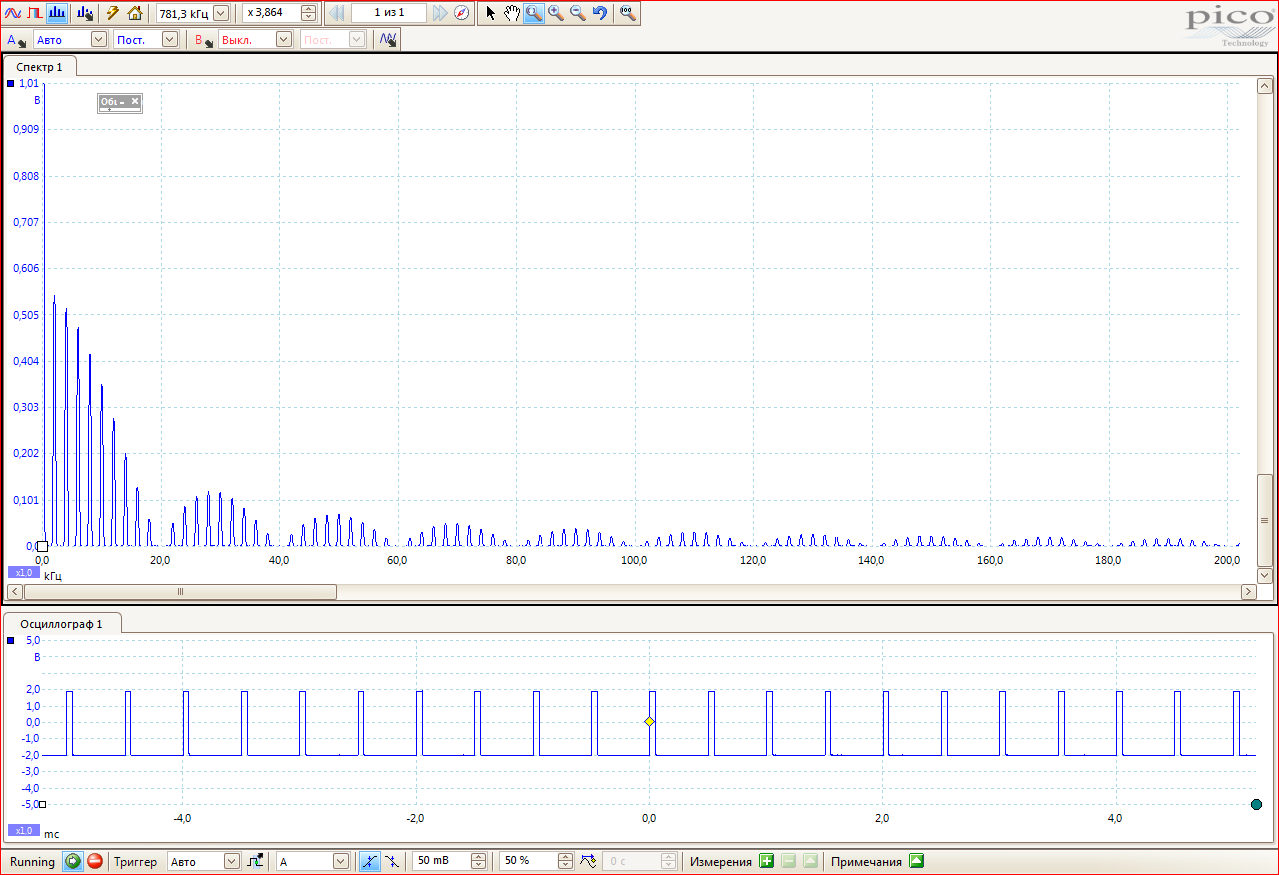
\includegraphics[width=0.5\pdfpagewidth]{Прямоугольный сигнал 2 кГц.PNG}
    \caption{Прямоугольный сигнал 2 кГц}
\end{figure}

\begin{figure}[h!]
    \centering
    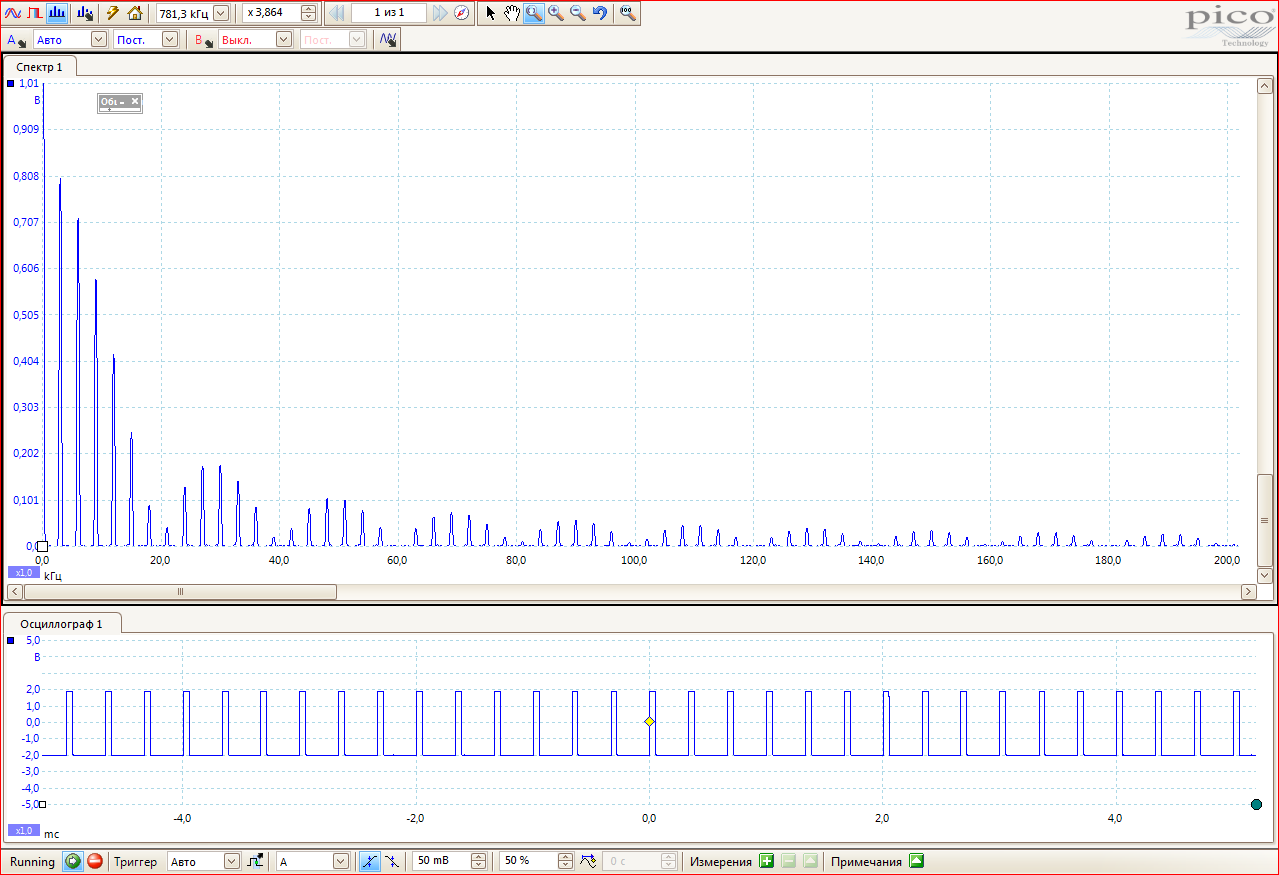
\includegraphics[width=0.5\pdfpagewidth]{Прямоугольный сигнал 3 кГц.PNG}
    \caption{Прямоугольный сигнал 3 кГц}
\end{figure}

\begin{figure}[h!]
    \centering
    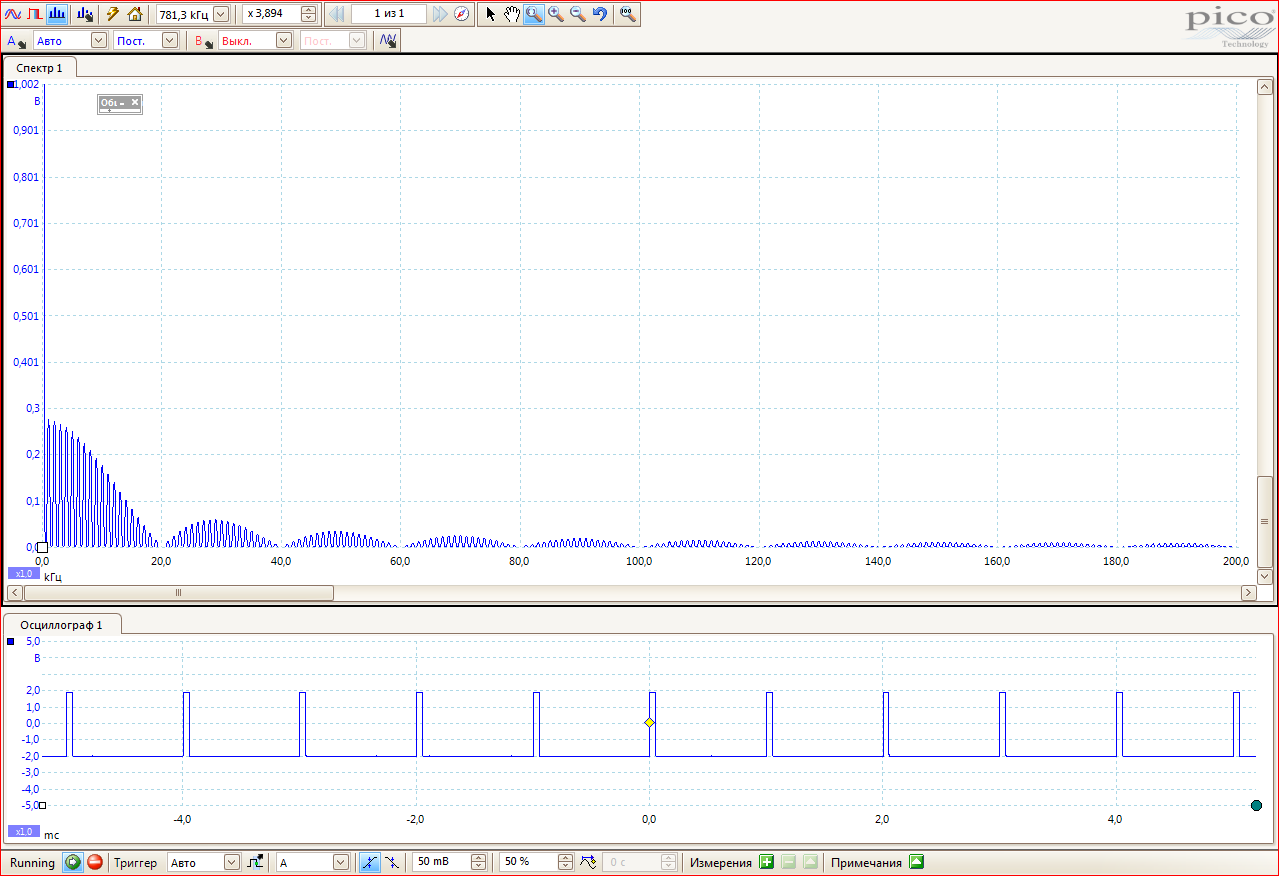
\includegraphics[width=0.5\pdfpagewidth]{Прямоугольный сигнал 1кГц 50 мкс.PNG}
    \caption{Прямоугольный сигнал $\tau$ = 50 мкс}
\end{figure}

\begin{figure}[h!]
    \centering
    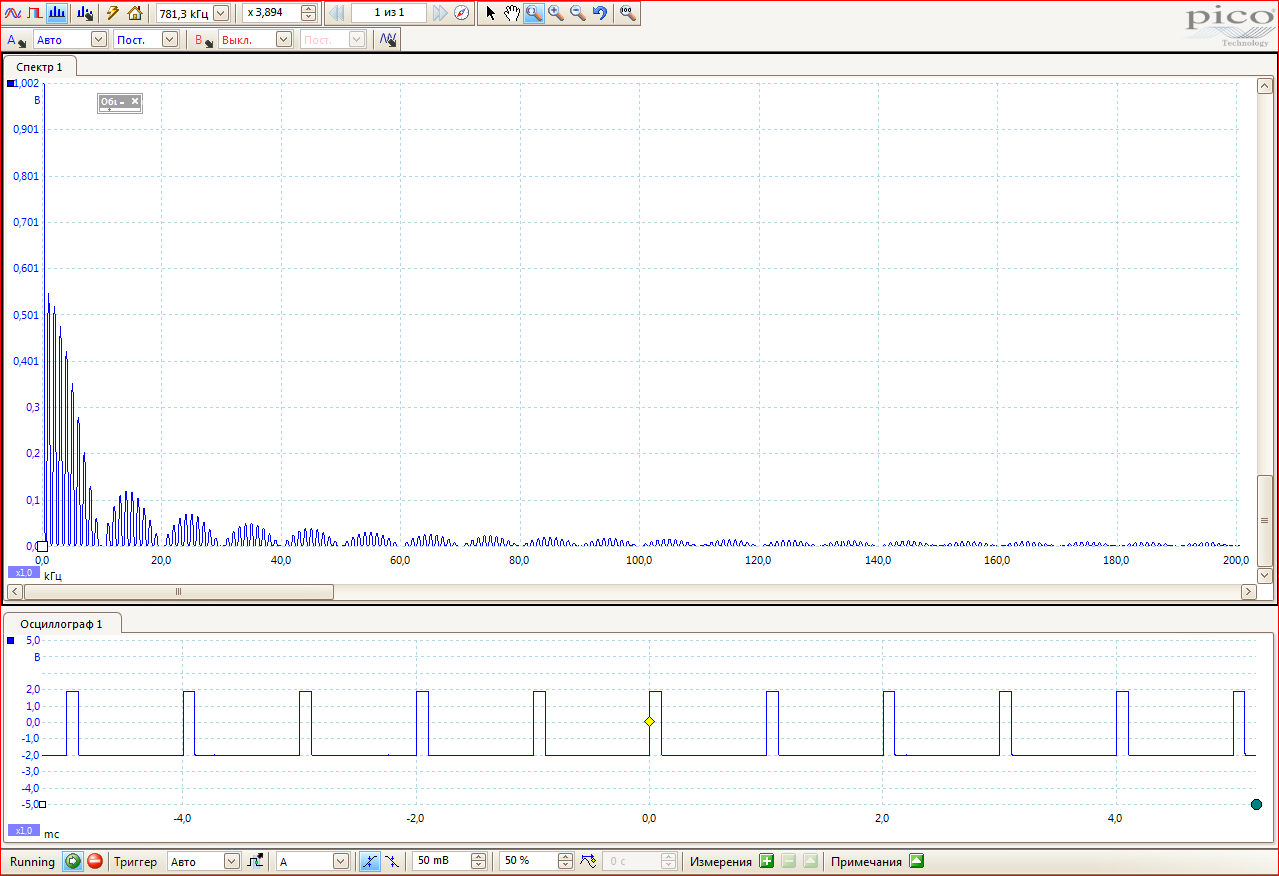
\includegraphics[width=0.5\pdfpagewidth]{Прямоугольный сигнал 1кГц 100 мкс.PNG}
    \caption{Прямоугольный сигнал $\tau$ = 100 мкс}
\end{figure}

\begin{figure}[h!]
    \centering
    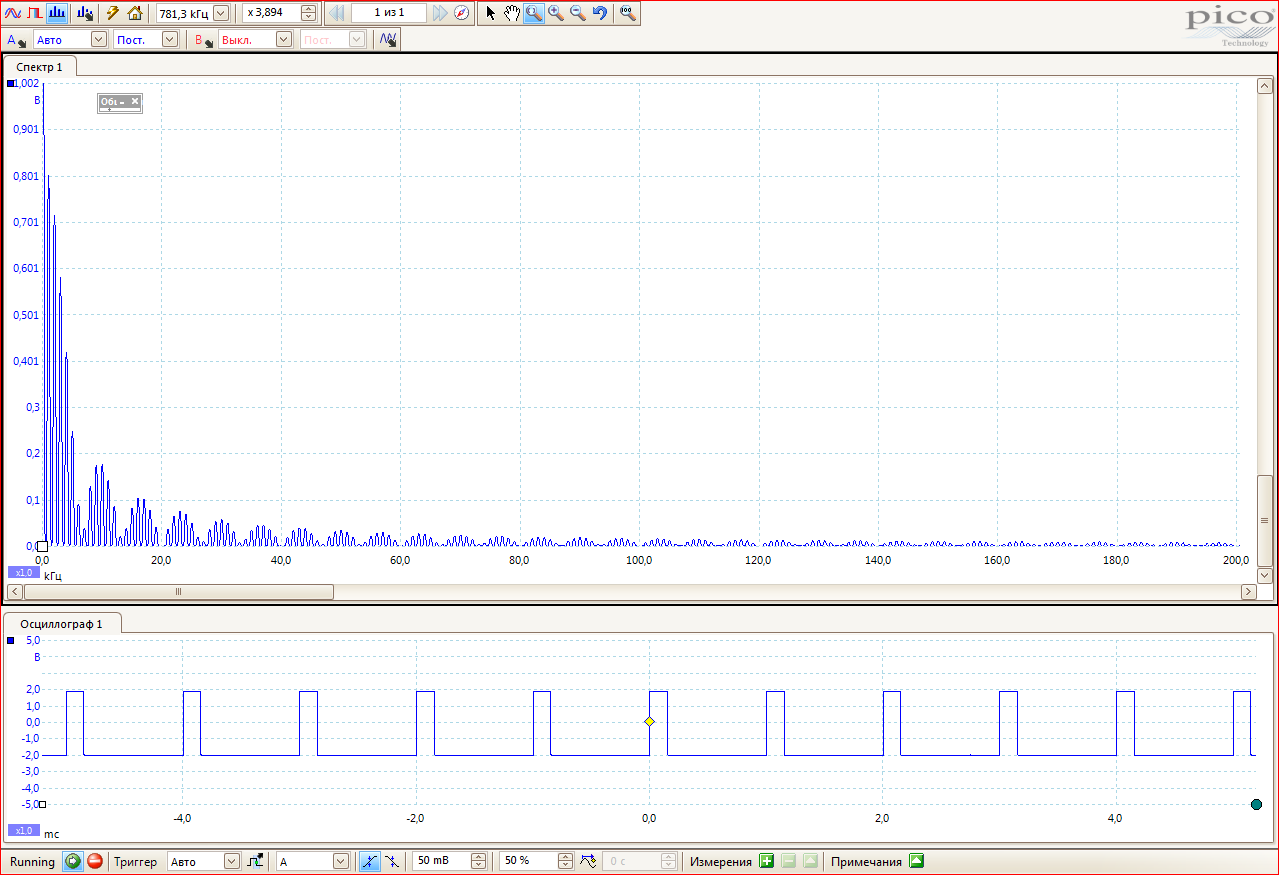
\includegraphics[width=0.5\pdfpagewidth]{Прямоугольный сигнал 1кГц 150 мкс.PNG}
    \caption{Прямоугольный сигнал $\tau$ = 150 мкс}
\end{figure}

\clearpage
\newpage

Как мы можем видеть, спектр находится в соответствии с формулой для гармоник
спектра прямоугольных сигналов:
\begin{equation}
    c_n = \frac {\tau}{T} \frac{\sin{n\omega_0 \tau / 2}}{n \omega \tau / 2}
\end{equation}

\subsection{Измерение амплитуд и частот гармоник}

При фиксированных параметрах $\nu_\text{повт}$ = 1 кГц и $\tau_\text{повт}$ = 50 мкс были измерены
амплитуды $a_n$ и частоты $\nu_n$ нескольких спектральных компонент (гармоник).
Эти значения были сопоставлены с теоретически рассчитанными на основе соотношений:

Поскольку единицы измерения амплитуд гармоник произвольны, для сравнения использовались относительные величины, например \( |a_n / a_1| \). Полученные экспериментальные данные занесены в таблицу \ref{table:1}.

\begin{table}[h!]
\centering
\begin{tabular}{|c|c|c|c|c|c|c|c|}
\hline
\( n \) & 1 & 2 & 3 & 4 & 5 & 6 & 7 \\ \hline
\( \nu_n^{\text{эксп}} \), Гц & 1 & 2 & 3 & 4 & 5 & 6 & 7 \\ \hline
\( \nu_n^{\text{теор}} \), Гц & 1 & 2 & 3 & 4 & 5 & 6 & 7 \\ \hline
\( |a_n|^{\text{эксп}}, \text{ усл. ед.} \) & 277 & 273 & 267 & 260 & 250 & 238 & 226 \\ \hline
\( |a_n / a_1|^{\text{эксп}} \) & 1.00 & 0.99 & 0.96 & 0.94 & 0.90 & 0.86 & 0.82 \\ \hline
\( |a_n / a_1|^{\text{теор}} \) & 1.00 & 0.99 & 0.97 & 0.94 & 0.90 & 0.86 & 0.81 \\ \hline
\end{tabular}
\label{table:1}
\caption{Измерение характеристик спектра прямоугольного сигнала}
\end{table}

Также были измерены ширины спектра, данные занесены в таблицу \ref{table:2}.

\begin{table}[h!]
\centering
\caption{Измерение ширины спектра $\nu = 1$ кГц, $\tau = 50$ мкс}
\label{table:2}
\begin{tabular}{|c|c|}
\hline
\( \tau \), мкс & \( \Delta \nu \), кГц \\ \hline
20 & 50 \\ \hline
60 & 16.6 \\ \hline
100 & 10 \\ \hline
150 & 6.6 \\ \hline
200 & 5 \\ \hline
\end{tabular}
\end{table}

Также были измерены расстояния между гармониками:


При фиксированной длительности импульса \( \tau = 100 \, \text{мкс} \) были проведены измерения расстояний \( \delta \nu = \nu_{n+1} - \nu_n \) между соседними гармониками спектра при изменении периода повторения \( T \) в диапазоне от \( 2\tau \) до \( 50\tau \), данные занесены в таблицу \ref{table:3}.

\begin{table}[h!]
\centering
\caption{Измерение расстояния между гармониками}
\label{table:3}
\begin{tabular}{|c|c|c|c|}
\hline
\( T \), мс & \( \nu_1 \), кГц & \( \nu_2 \), кГц & \( \Delta \nu \), кГц \\ \hline
1 & 1.0 & 2.0 & 1.0 \\ \hline
2 & 1.0 & 1.5 & 0.4 \\ \hline
3 & 1.0 & 1.4 & 0.4 \\ \hline
4 & 1.7 & 2.0 & 0.4 \\ \hline
5 & 1.4 & 1.6 & 0.2 \\ \hline
\end{tabular}
\end{table}

% \subsection{Графики зависимостей ширины спектра от расстояния между гармониками}

\section{Анализ спектра синусоидального импульса}

Был настроен генератор сигнала с несущей частототй $\nu_0 = 50$ кГц, 
периодом повторения \( T = 1 \, \text{мc} \) и числом периодов в одном импульсе \( N = 5 \ \)

Отсюда следует, что $\nu_\text{повт} = 1/T = 1$ кГц

А длительность импульса \( \tau = N / \nu_0 = 100 \ \text{мкс} \)

Посмотрим на сигналы и спектры при стандартных параметрах, а также при из изменении 

\begin{figure}[h!]
\centering
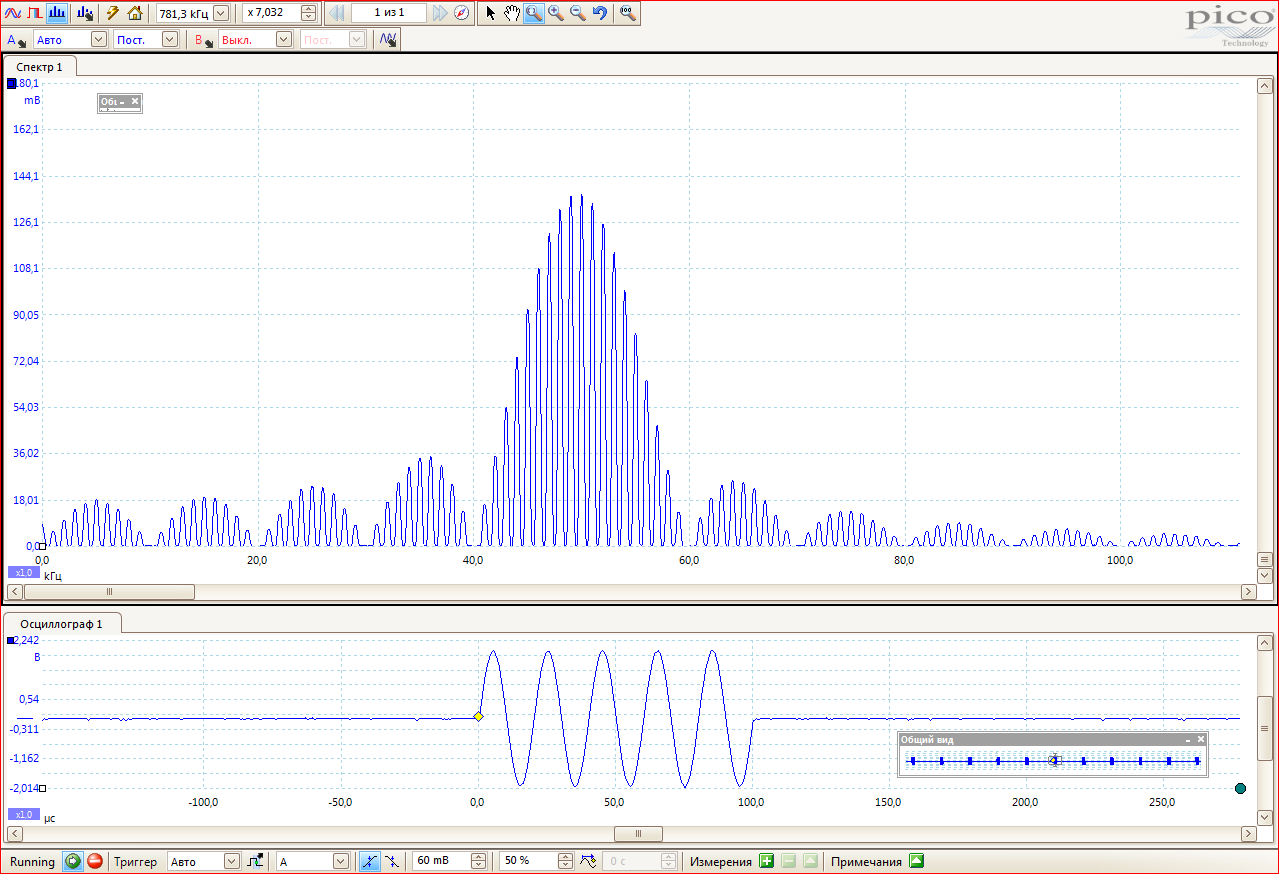
\includegraphics[width=0.8\textwidth]{Цуг стандарт.PNG}
\caption{Синусоидальный импульс, стандартные параметры}
\end{figure}

\begin{figure}[h!]
\centering
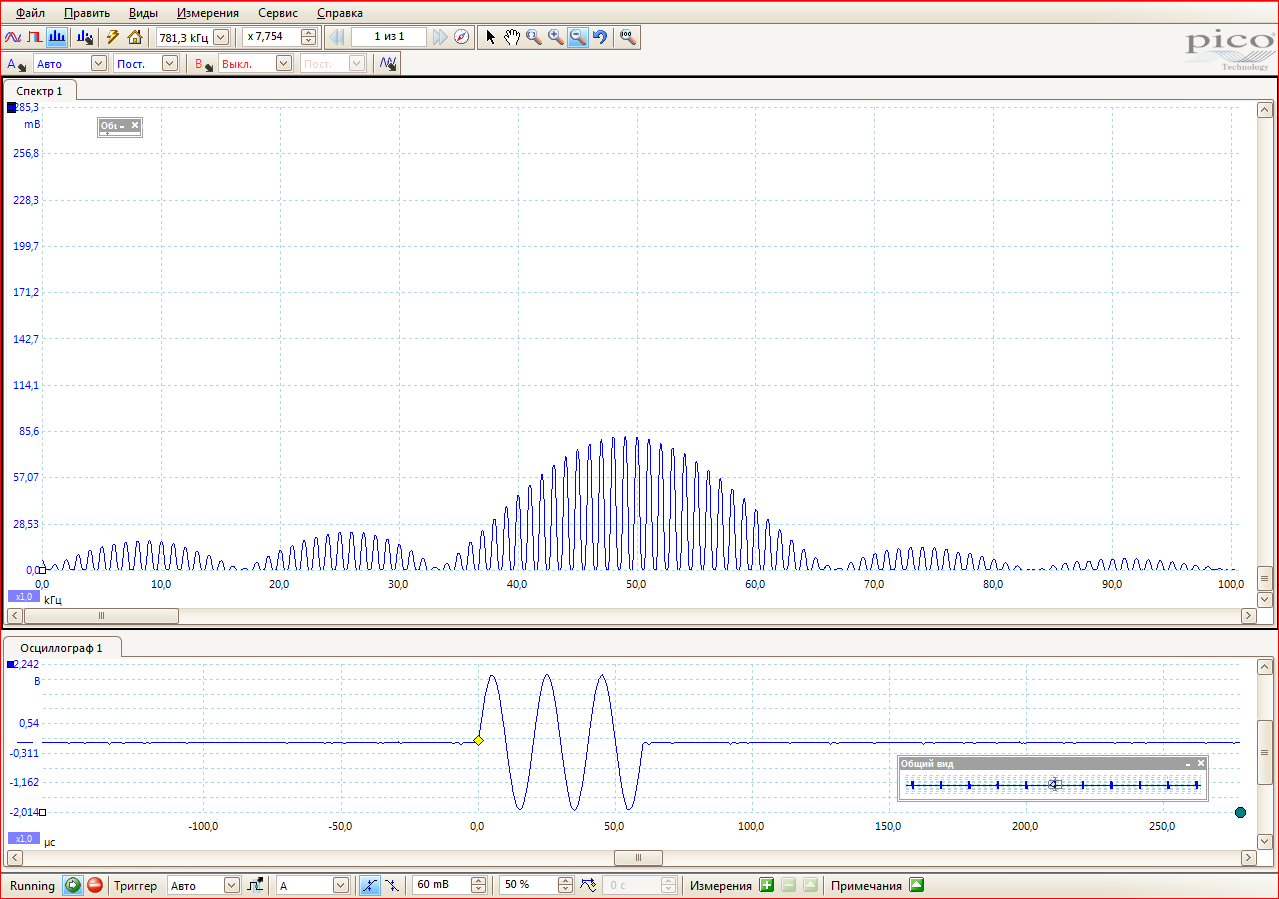
\includegraphics[width=0.8\textwidth]{Цуг n=3.PNG}
\caption{Синусоидальный импульс. $N = 3$}
\end{figure}

\begin{figure}[h!]
\centering
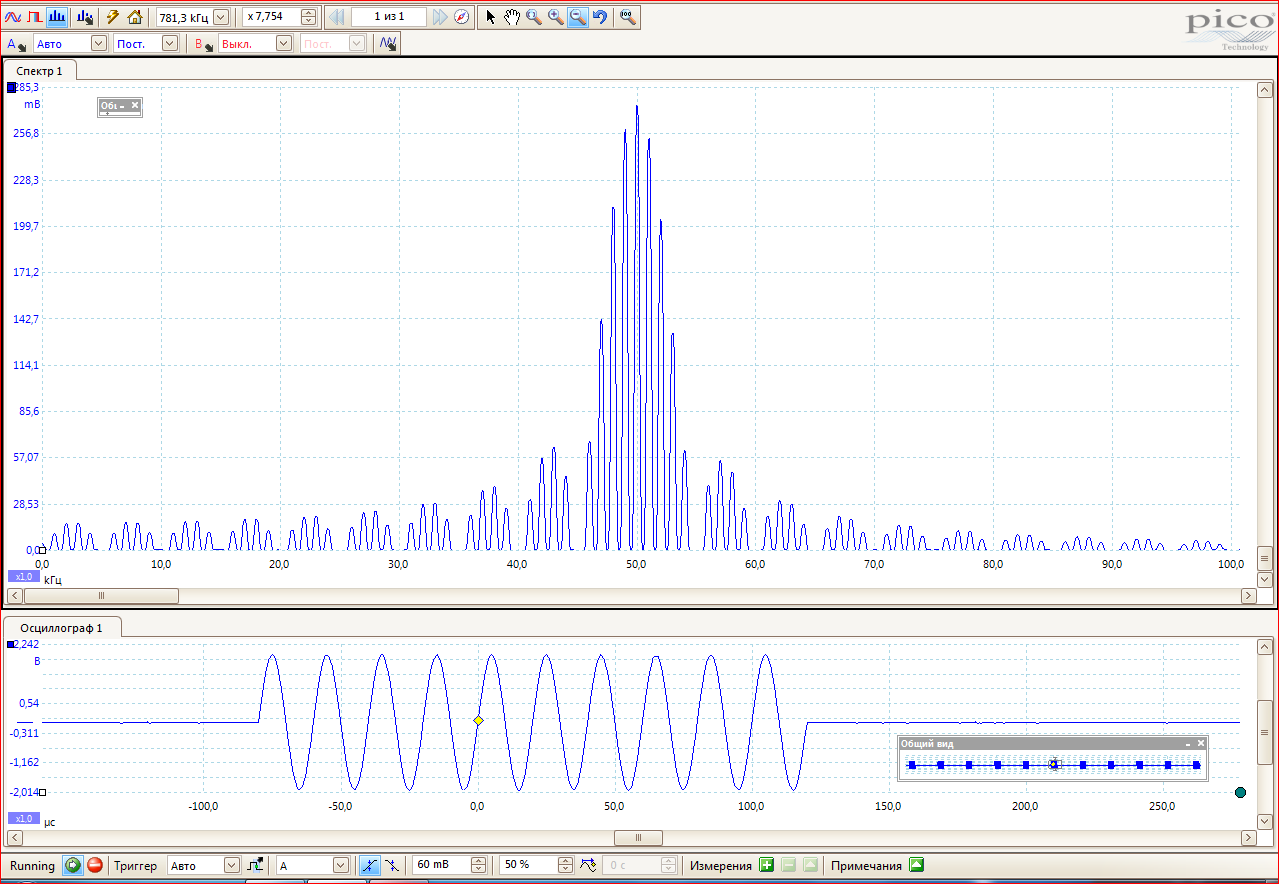
\includegraphics[width=0.8\textwidth]{Цуг n=10.PNG}
\caption{Синусоидальный импульс. $N = 10$}
\end{figure}

\begin{figure}[h!]
\centering
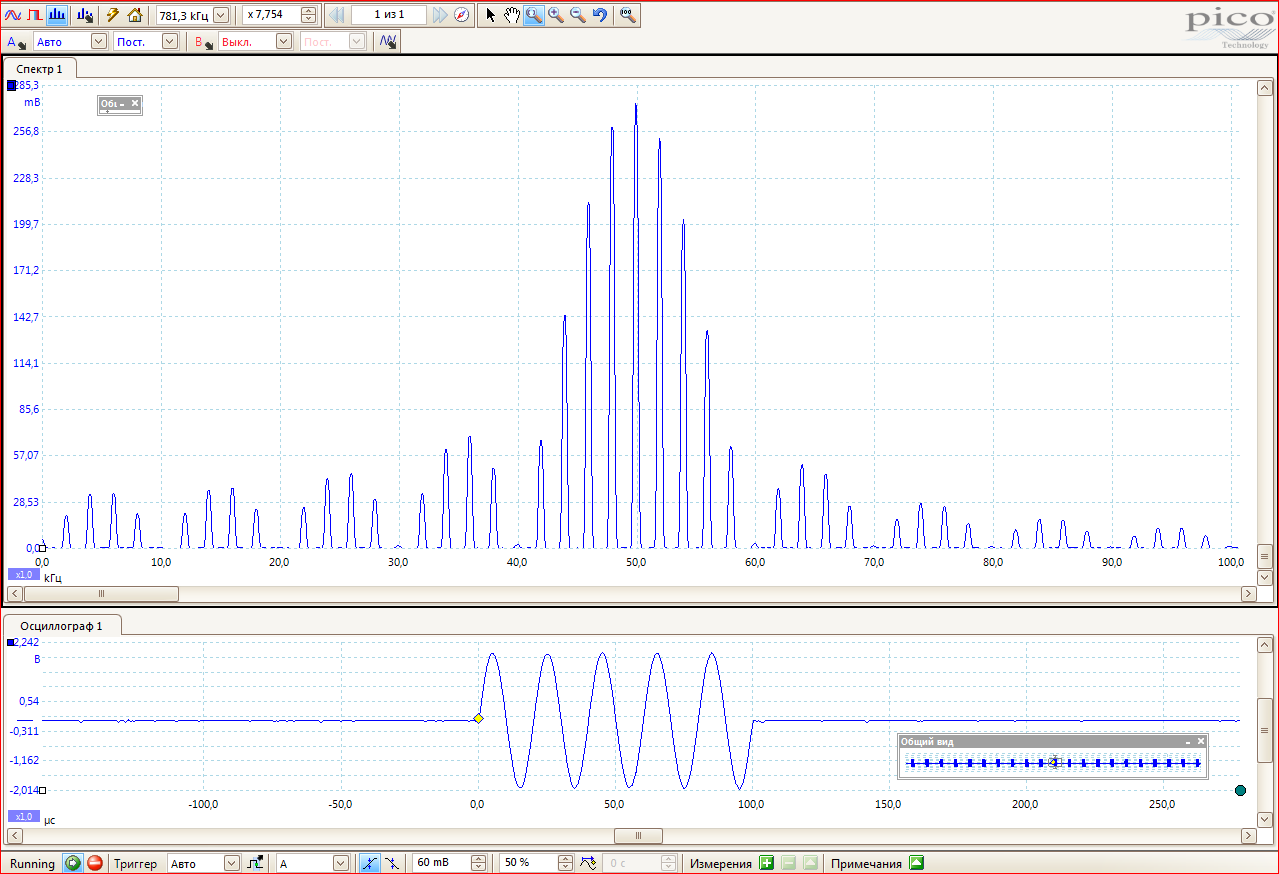
\includegraphics[width=0.8\textwidth]{Цуг т=500.PNG}
\caption{Синусоидальный импульс. $T = 500$ мкс}
\end{figure}

\begin{figure}[h!]
\centering
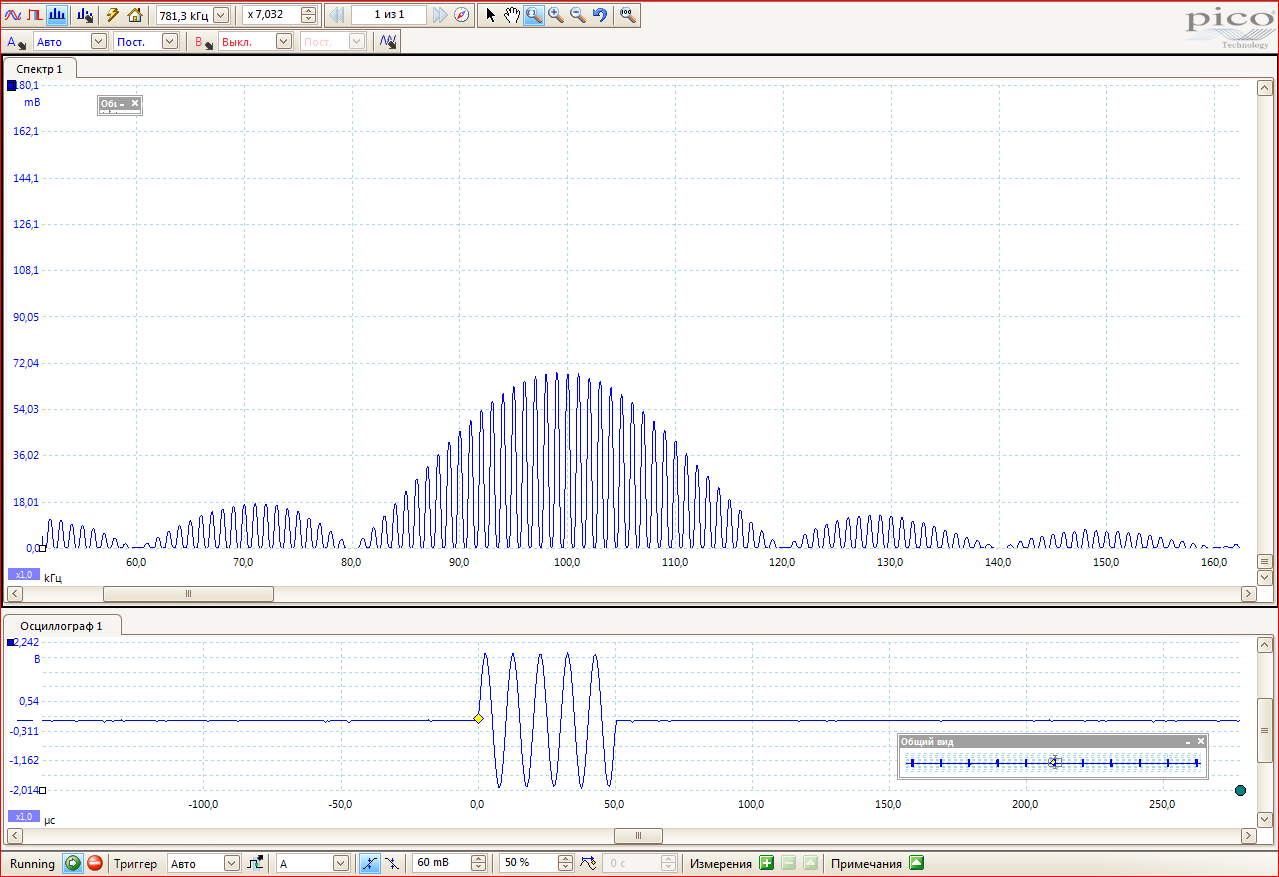
\includegraphics[width=0.8\textwidth]{Цуг 100кГц.PNG}
\caption{Синусоидальный импульс. $\nu_\text{повт} = 10$ кГц}
\end{figure}

Результаты соответствуют теоретическим данным.

\begin{equation}
    c_n(\omega) = \frac{\tau}{2} \frac{\sin{(n\omega_0 \tau / 2)}}{n \omega \tau / 2}
\end{equation}

\clearpage
\newpage

\section{Спект амплитудно-модулированного синусоидального сигнала}

Был настроен режим генерации амплитудно-модулированного синусоидального сигнала
с $\nu_0 = 50$ кГц, частотой модуляции $\nu_\text{мод} = 2$ кГц, глубиной модуляции $m = 50\%$

Было проверено соотношение $ m = \frac{A_{max} - A_{min}}{A_{max} + A_{min}} $,
$A_{max} = 1.49B$, $A_{min} = 0.49B$, $m \approx 0.5$ - соотношение выполняется

\begin{figure}[h!]
\centering
\includegraphics[width=0.8\textwidth]{АМ.PNG}
\caption{А-м импульс. Стандартные параметры}
\end{figure}

\begin{figure}[h!]
\centering
\includegraphics[width=0.8\textwidth]{АМ nu=40k.PNG}
\caption{А-м импульс. $\nu = 40$ кГц}
\end{figure}

\begin{figure}[h!]
\centering
\includegraphics[width=0.8\textwidth]{АМ nu=60k.PNG}
\caption{А-м импульс. $\nu = 60$ кГц}
\end{figure}

\begin{figure}[h!]
\centering
\includegraphics[width=0.8\textwidth]{АМ nu_mod=1k.PNG}
\caption{А-м импульс. $\nu_\text{мод} = 1$ кГц}
\end{figure}

\begin{figure}[h!]
\centering
\includegraphics[width=0.8\textwidth]{АМ nu_mod=3k.PNG}
\caption{А-м импульс. $\nu_\text{мод} = 3$ кГц}
\end{figure}

\begin{figure}[h!]
\centering
\includegraphics[width=0.8\textwidth]{АМ nu_mod=8k.PNG}
\caption{А-м импульс. $\nu_\text{мод} = 8$ кГц}
\end{figure}

\clearpage
\newpage

\subsection{Измерение отношения амплитуд боковых и основной гармоник}

Изменяя на генераторе глубину модуляции m в диапазоне от $10\%$ до
$100\%$, измерим отношение амплитуд боковой гармоники ($a_\text{бок}$) к основной гармонике ($a_\text{осн}$)

\begin{figure}[h!]
\centering
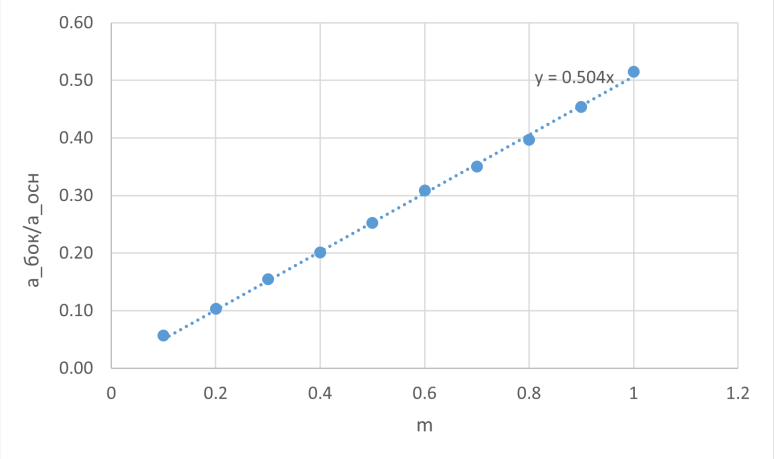
\includegraphics[width=0.8\textwidth]{aboba.png}
\caption{Зависимостьь отношения амплитуд боковых и основной гармнок}
\end{figure}

Из графика: $k = 0.50 \pm 0.01$ - что сходится с теорией

\clearpage
\newpage

\subsection*{Е. Изучение фильтрации сигналов}

Для RC-фильтра низких частот рассчитаем его характерную временную постоянную:

\begin{equation}
    \tau_{RC} = R \cdot C = 3 ~ \text{мкс}
\end{equation}

На вход интегратора были поданы прямоугольныe импульсы с периодом повторения $T \approx \tau_{RC}$, 
$\tau \approx T / 20$

Для разных $T$ посмотрим спектр и сигнал на выходе фильтра

\begin{figure}[h!]
\centering
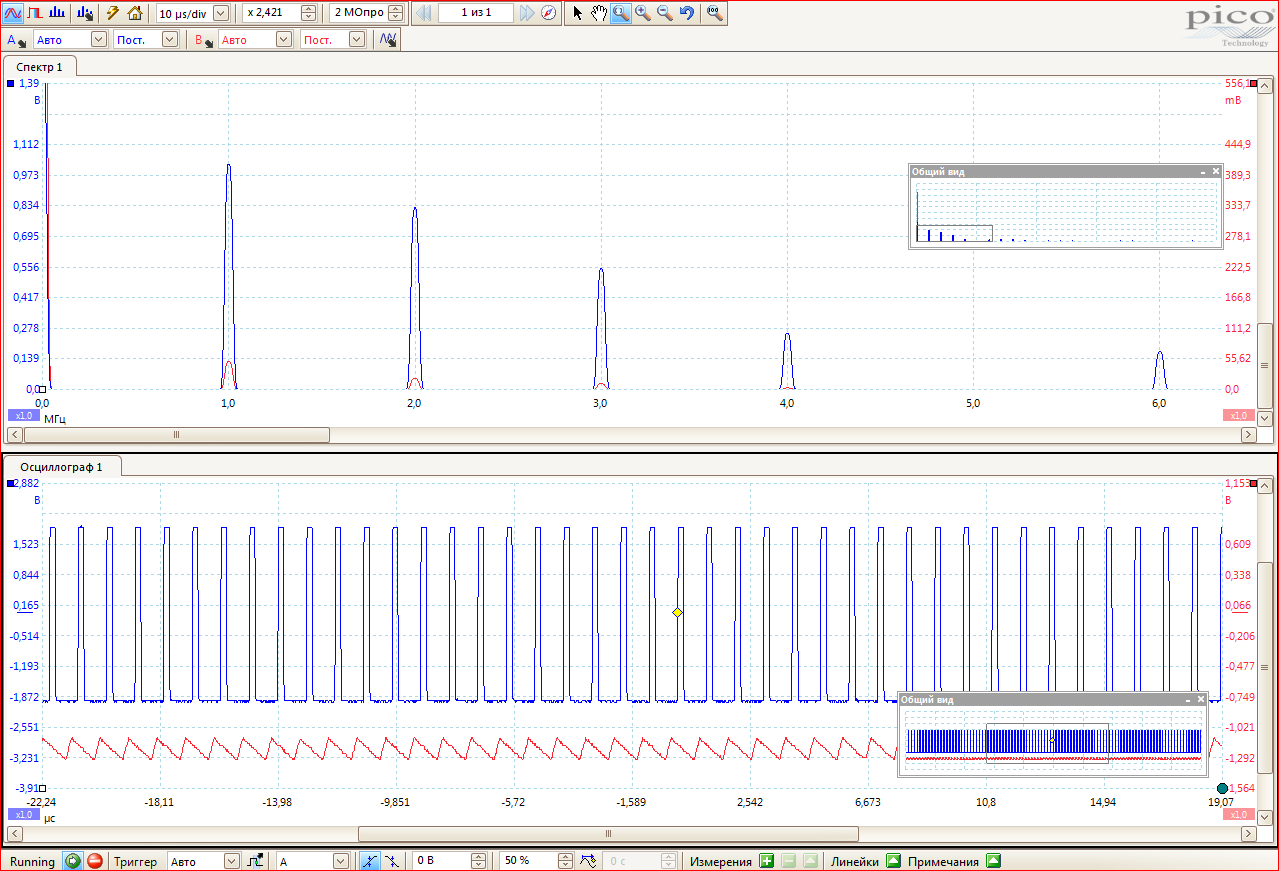
\includegraphics[width=0.8\textwidth]{Интегратор tau=200нс T=1мкс.PNG}
\caption{Выход RC-цепочки. T = 1мкс}
\end{figure}

\begin{figure}[h!]
\centering
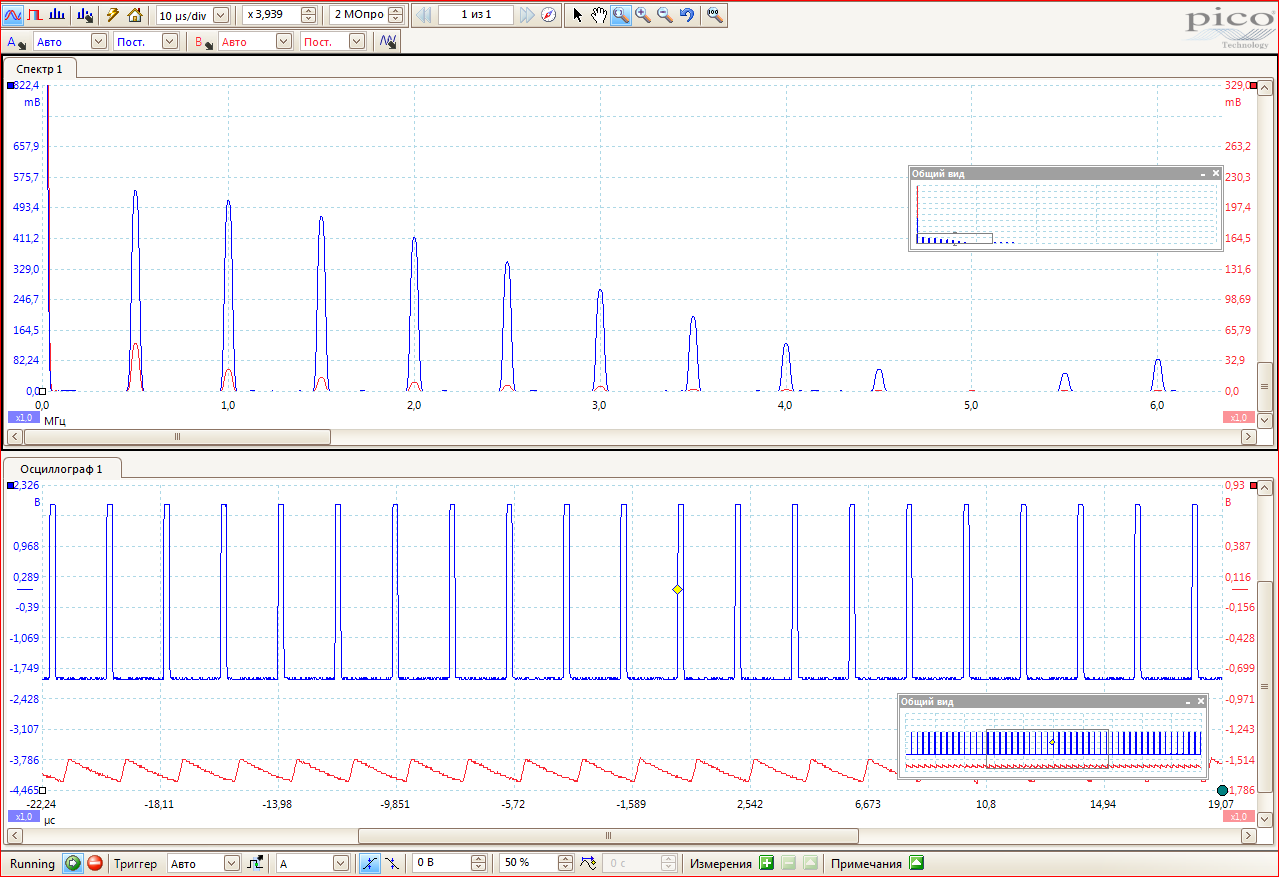
\includegraphics[width=0.8\textwidth]{Интегратор tau=200нс T=2мкс.PNG}
\caption{Выход RC-цепочки. T = 2мкс}
\end{figure}

\begin{figure}[h!]
\centering
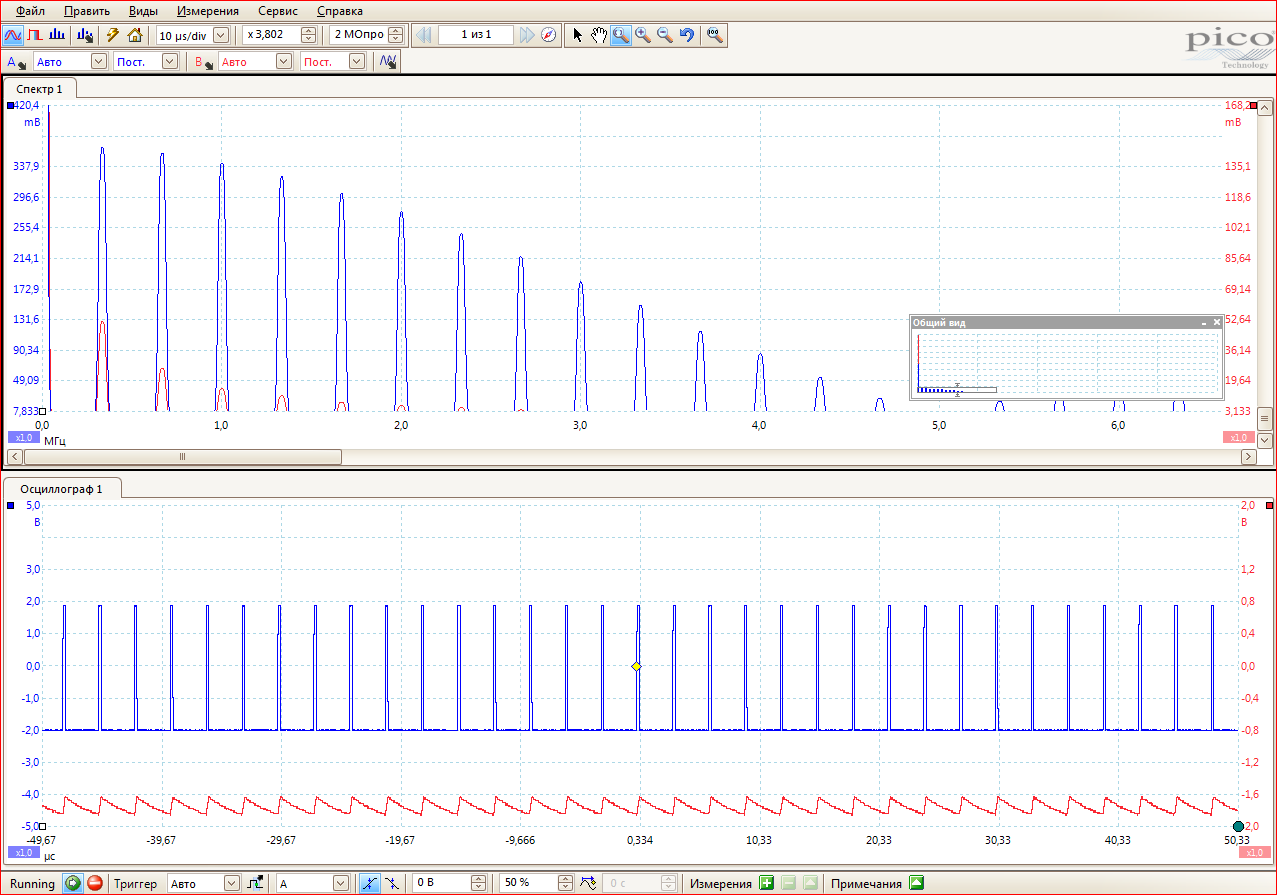
\includegraphics[width=0.8\textwidth]{Интегратор tau=200нс T=3мкс.PNG}
\caption{Выход RC-цепочки. T = 3мкс}
\end{figure}

\clearpage
\newpage

\subsection{Измерение отношений амплитуд спектральных гармоник}

При фиксированном значении периода T были проведены измерения 
отношений амплитуд соответствующих спектральных гармоник фильтрованного сигнала и исходного сигнала для 5 гармоник.
Отношение амплитуд для n-й гармоники:

\begin{table}[h!]
\centering
\begin{tabular}{|c|c|c|c|}
\hline
$\nu$, kГц & $|a_n^{\phi}|$, МB & $|a_n^0|$, мB & $K_n$ \\
\hline
333  & 359.2  & 1019  & 0.35 \\
666  & 154.6  & 827.6 & 0.18 \\
1000 & 59.11  & 545.6 & 0.11 \\
1333 & 22.26  & 256.1 & 0.087 \\
2333 & 11.09  & 236.4 & 0.047 \\
\hline
\end{tabular}
\caption{Измерение отношения амплитуд спектров входного и выходного сигналов}
\end{table}

\begin{equation}
    K_n = | \frac{a_n^\Phi}{a_n^0} |
\end{equation}

На основе проведённых измерений был построен график зависимости амплитудного коэффициента фильтрации $K(\nu)$
от величины, обратной частоте

\begin{figure}[h!]
\centering
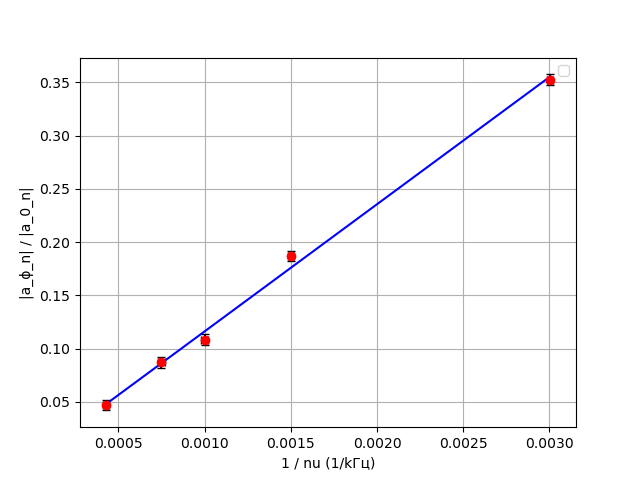
\includegraphics[width=0.8\textwidth]{graph.png}
\caption{}
\end{figure}

Из полученного графика можно найти его коэффициент наклона:

\begin{equation}
    k = \frac{1}{2\pi RC} = (59 \pm 1) \text{кГц}
\end{equation}

Отсюда: $RC = (2.70 \pm 0.05)$ - близко, но не совсем точно

Скорее всего это произошло из-за аппроксимации прямой

\newpage
\cleanpage

\section{Вывод}

В ходе работы были изучены различные сигнали и их спектры, а также влияние на них параметров

\end{document}

